\documentclass{beamer}
\usepackage[english,russian]{babel}   % руссификации AmSLaTeX
\usetheme{CambridgeUS}

\usepackage{amsmath,amsfonts,amssymb,euscript,graphicx,wrapfig,multirow,mathtools,amsthm}
\usepackage{dsfont}

%%% Работа с картинками
\usepackage{graphicx}  % Для вставки рисунков
\graphicspath{{./images/}}  % папки с картинками
\setlength\fboxsep{3pt} % Отступ рамки \fbox{} от рисунка
\setlength\fboxrule{1pt} % Толщина линий рамки \fbox{}
\usepackage{wrapfig} % Обтекание рисунков и таблиц текстом
\usepackage[export]{adjustbox}
\usepackage{caption}
\captionsetup[figure]{labelsep=space}
\usepackage{subcaption}
\usepackage{float}
\usepackage{tikz-cd}
\usetikzlibrary{babel}
\usepackage{animate}
\usepackage{tabularx}

\usepackage{csquotes} % biblatex рекомендует его подключать. Пакет для оформления сложных блоков цитирования.
\usepackage[%
backend=biber,% движок
bibencoding=utf8,% кодировка bib файла
sorting=none,% настройка сортировки списка литературы
style=gost-numeric,% стиль цитирования и библиографии (по ГОСТ)
language=autobib,% получение языка из babel/polyglossia, default: autobib % если ставить autocite или auto, то цитаты в тексте с указанием страницы, получат указание страницы на языке оригинала
autolang=other,% многоязычная библиография
clearlang=true,% внутренний сброс поля language, если он совпадает с языком из babel/polyglossia
sortcites=true,% сортировать номера затекстовых ссылок при цитировании (если в квадратных скобках несколько ссылок, то отображаться будут отсортированно, а не абы как)
doi=false,% Показывать или нет ссылки на DOI
isbn=false,% Показывать или нет ISBN, ISSN, ISRN
eprint=false
]{biblatex}
\renewcommand*{\mkbibhdnamefamily}[1]{#1}
\renewcommand*{\multicitedelim}{\addcomma\space}
\renewcommand*{\newblockpunct}{\addperiod\addnbspace\cyrdash\space\bibsentence}
\DeclareSourcemap{
	\maps{
		\map[overwrite]{ % переделка формата записи даты
			\step[fieldsource=urldate,
			match=\regexp{([0-9]{2})\.([0-9]{2})\.([0-9]{4})},
			replace={$3-$2-$1$4}, % $4 вставлен исключительно ради нормальной работы программ подсветки синтаксиса, которые некорректно обрабатывают $ в таких конструкциях
			final]
}}}
\addbibresource{author.bib}
\renewcommand*{\bibfont}{\small}
%%%END

%Algorithms
%http://blog.harrix.org/article/648
\usepackage[vlined, ruled]{algorithm2e}

\SetKwInput{KwData}{Исходные данные}
\SetKwInput{KwResult}{Результат}
\SetKwInput{KwIn}{Входные данные}
\SetKwInput{KwOut}{Выходные данные}
\SetKwIF{If}{ElseIf}{Else}{если}{тогда}{иначе если}{иначе}{конец условия}
\SetKwFor{While}{до тех пор, пока}{выполнять}{конец цикла}
\SetKw{KwTo}{от}
\SetKw{KwRet}{возвратить}
\SetKw{Return}{возвратить}
\SetKwBlock{Begin}{начало блока}{конец блока}
\SetKwSwitch{Switch}{Case}{Other}{Проверить значение}{и выполнить}{вариант}{в противном случае}{конец варианта}{конец проверки значений}
\SetKwFor{For}{цикл}{выполнять}{конец цикла}
\SetKwFor{ForEach}{Для каждой}{выполнять}{Конец цикла}
\SetKwRepeat{Repeat}{повторять}{до тех пор, пока}
\SetAlgorithmName{Алгоритм}{алгоритм}{Список алгоритмов}

\DeclareMathOperator{\im}{im}
\DeclarePairedDelimiter\norm{\lVert}{\rVert}%
\newcommand{\quotient}[2]{{\raisebox{.2em}{$#1$}\left/\raisebox{-.2em}{$#2$}\right.}}

\makeatother
\setbeamertemplate{footline}
{
	\leavevmode%
	\hbox{%
		\begin{beamercolorbox}[wd=.8\paperwidth,ht=2.25ex,dp=1ex,center]{title in head/foot}%
			\usebeamerfont{title in head/foot}\insertshorttitle
		\end{beamercolorbox}%
		\begin{beamercolorbox}[wd=.2\paperwidth,ht=2.25ex,dp=1ex,center]{date in head/foot}%
			\insertframenumber{} / \inserttotalframenumber\hspace*{1ex}
	\end{beamercolorbox}}%
	\vskip0pt%
}
\makeatletter

\title{Применение персистентных гомологий для задачи классификации изображений}

\author{\small Обучающийся \qquad\qquad\qquad\qquad\qquad Снопов П.М.\\
		\enspace Руководитель \qquad  д.т.н., проф. \qquad Леденева Т.М.}
\institute[ВГУ]{{ Воронежский Государственный Университет} \\ 
				Факультет прикладной математики, информатики и механики \\[1em]
				Кафедра вычислительной математики и прикладных \\
				информационных технологий}

\date{\footnotesize Бакалаврская работа \\
	  Направление 01.03.02 Прикладная математика и информатика \\
  	  Профиль Математическое моделирование и вычислительная математика}


\begin{document}
	\begin{frame}[plain]
		\centering
		
		\begin{beamercolorbox}[sep=8pt,center,colsep=-4bp,rounded=true,shadow=true]{institute}
			\usebeamerfont{institute}\insertinstitute
		\end{beamercolorbox}
		
		{\usebeamercolor[fg]{titlegraphic}\inserttitlegraphic\par}
		
		\begin{beamercolorbox}[sep=8pt,center,colsep=-4bp,rounded=true,shadow=true]{title}
			\usebeamerfont{title}\inserttitle\par%
			\ifx\insertsubtitle\@empty%
			\else%
			\vskip0.25em%
			{\usebeamerfont{subtitle}\usebeamercolor[fg]{subtitle}\insertsubtitle\par}%
			\fi%     
		\end{beamercolorbox}%
		
		\vskip1em\par
		
		\begin{beamercolorbox}[sep=8pt,center,colsep=-4bp,rounded=true,shadow=true]{date}
			\usebeamerfont{date}\insertdate
		\end{beamercolorbox}\vskip0.5em
		
		\begin{beamercolorbox}[sep=8pt,center,colsep=-4bp,rounded=true,shadow=true]{author}
			\usebeamerfont{author}\insertauthor
		\end{beamercolorbox}
		\note{Здравствуйте, уважаемая комиссия! Меня зовут Снопов Павел, мой научный руководитель -- Леденева Татьяна Михайловна, тема моей бакалаврской работы -- применение персистентных гомологий для задачи классификации изображений.}
	\end{frame}
	\footnotesize
	\section{Введение}
	
	\subsection{Актуальность}	
		\begin{frame}
			\frametitle{Актуальность}
			\begin{itemize}
				\item Классификация изображений -- фундаментальная задача анализа данных, одно из основных направлений приложения машинного обучения к компьютерному зрению.%, которое в последнее время имеет очень интенсивное развитие, связанное с достижениями нейронных сетей.
				\item Машинное обучение -- главный тренд последних 10 лет($\sim 150$ публ./день).
				\item Устойчивые гомологии и топологический анализ данных -- недавно возникшая и быстро развивающаяся область современной математики и анализа данных.
			\end{itemize}
			\note{Несколько слов об актуальности: ...}
		\end{frame}
	
		\subsection{Постановка задачи}
		\begin{frame}
			\frametitle{Постановка задачи}
			\begin{columns}[] % align columns
				\begin{column}{.5\textwidth}
				\begin{itemize}
					\item Задано конечное множество объектов вместе с метками классов. 
					\item Метки классов остальных объектов не известны. 
					\item Требуется построить алгоритм, способный классифицировать произвольный объект из исходного множества.
				\end{itemize}
				\end{column}%
			\hfill%
				\begin{column}{.49\textwidth}
					\begin{figure}
						\centering
						
\includegraphics[width=0.6\linewidth]{mnist_example.png}
						\caption{Пример изображения из датасета MNIST}
					\end{figure}
				\end{column}%
			\end{columns}
		\note{Имеется следующая задача: задано конечное множество объектов вместе с метками класса, а также заданы объекты без меток класса. Необходимо построить алгоритм, способный классифицировать объект исходного множества.}
		\end{frame}
	
		\subsection{Цель и задачи работы}
		\begin{frame}
		\frametitle{Цель и задачи работы}
			\textbf{\small Цель:} Исследование подхода, основанного на топологическом анализе данных, для классификации изображений \\[1em]
			\textbf{\small Задачи:}
			\begin{itemize}
				\item Изучение теоретических и практических основ топологического анализа данных
				\item Анализ подходов классификации изображений
				\item Формирование алгоритма на основе персистентных гомологий
				\item Проведение вычислительного эксперимента, выявление области применимости, плюсов и минусов данного подхода
			\end{itemize}
		\note{Цель: ..., задачи представлены на слайде}
		\end{frame}

	\section{Теоретические сведения}
	
		\subsection{Симплициальные комплексы}
		\begin{frame}
			\frametitle{Симплициальные комплексы}

				{\it Симплициальный комплекс $K$} -- это множество симплексов, т.е. выпуклых оболочек набора $n+1$ точек $\in \mathbb{R}^p$, таких, что векторы $ x_1 - x_0, ..., x_n - x_0 $ линейно независимы, при этом
				\begin{itemize}
					\setlength{\itemsep}{-1mm}
					\item Для каждого симплекса из $K$ его грани тоже лежат в $K$,
					\item Пересечение любых двух симплексов $\sigma, \tau \in K$ либо пусто, либо является гранью и $\sigma$, и $\tau$.
				\end{itemize}
			\begin{figure}
				\centering
				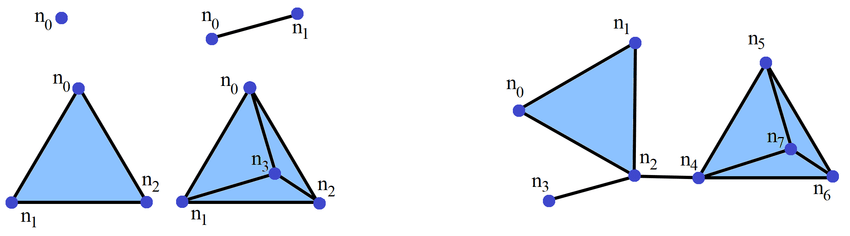
\includegraphics[width=\linewidth]{simplexAndComplex.png}
			\end{figure}
		\note{Основной объект в ТДА -- симплициальный комплекс. С.К. -- это множество правильно склеенных между собой симплексов, симплекс же -- это обобщение треугольника на большие размерности, например тетраэдр -- это симплекс.}
		\end{frame}
		\subsection{Cимплициальные гомологии}
		\begin{frame}[fragile]
			\frametitle{Симплициальные гомологии}
			{\it Группа симплициальных гомологий $H_n(K)$} размерности $n$ отражает количество {$n$-циклов}. Ранг данной группы -- {\it $n$-ое число Бетти} $\beta_n$ -- количество $n$-циклов.
			\[
				\beta_n = \mathrm{dim}(H_n(K))
			\]
			%Для симплициального комплекса можно посчитать его группы симплициальных гомологий $H_n$. Ранк $n$-ой группы -- это $n$-ое число Бетти $\beta_n$. Оно отражает количество $n$-мерных особенностей комплекса. Для $n=0$, $\beta_0$ отражает количество компонент связности данного пространства. При $n=1$ -- количество циклов. При $n=2$ число Бетти $\beta_2$ описывает количество "полостей".
			
			\begin{figure}[!htbp]
				\centering
				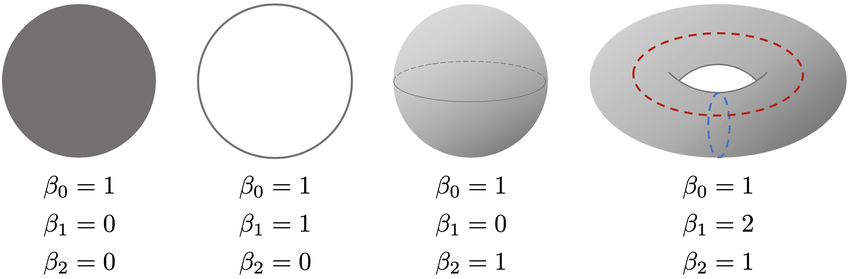
\includegraphics[width=\linewidth, keepaspectratio=true]{betti_numbers.png}
			\end{figure}
		\note{Для симплициального комплекса можно найти его группу $n$ симплициальных гомологий. Эта группа, а точнее ее ранг, число Бетти, характеризует количество $n$-циклов. При $n=0$ -- это количество компонент связности, $n=1$ -- количество циклов, как в теории графов и тд}
		\end{frame}
		
		\subsection{Фильтрации и устойчивые гомологии}
		\begin{frame}
			\frametitle{Как построить симплициальный комплекс?}
			\begin{figure}
				\centering
				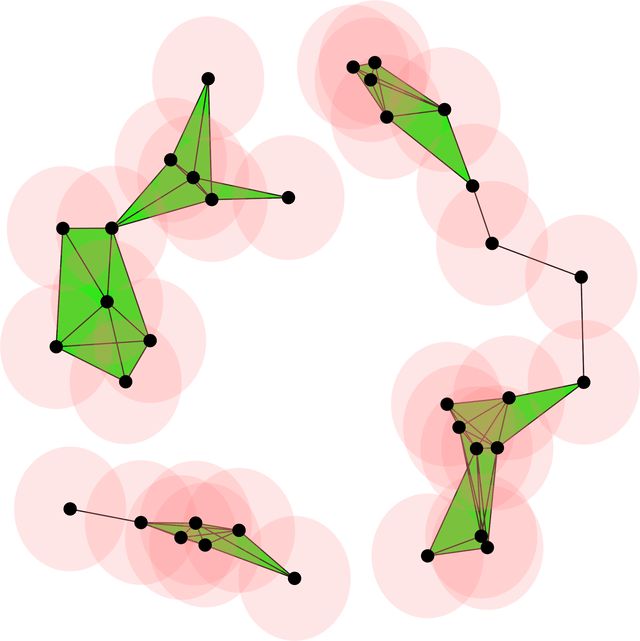
\includegraphics[width=0.6\linewidth, keepaspectratio=true]{vr.png}
			\end{figure}
		\note{Мы рассматриваем окрестность в каждой точке и смотрим, как окрестности пересекаются. Если n окрестностей пересекаются, то на соответствующие n точек натягиваем n-симплекс}
		\end{frame}
		\begin{frame}
			\frametitle{Фильтрации и устойчивые гомологии}
			{\it Фильтрация} -- коллекция комплексов. 
			
			{\it Устойчивые гомологии} -- коллекция групп гомологий комплексов фильтрации.
			\begin{figure}
				\centering
				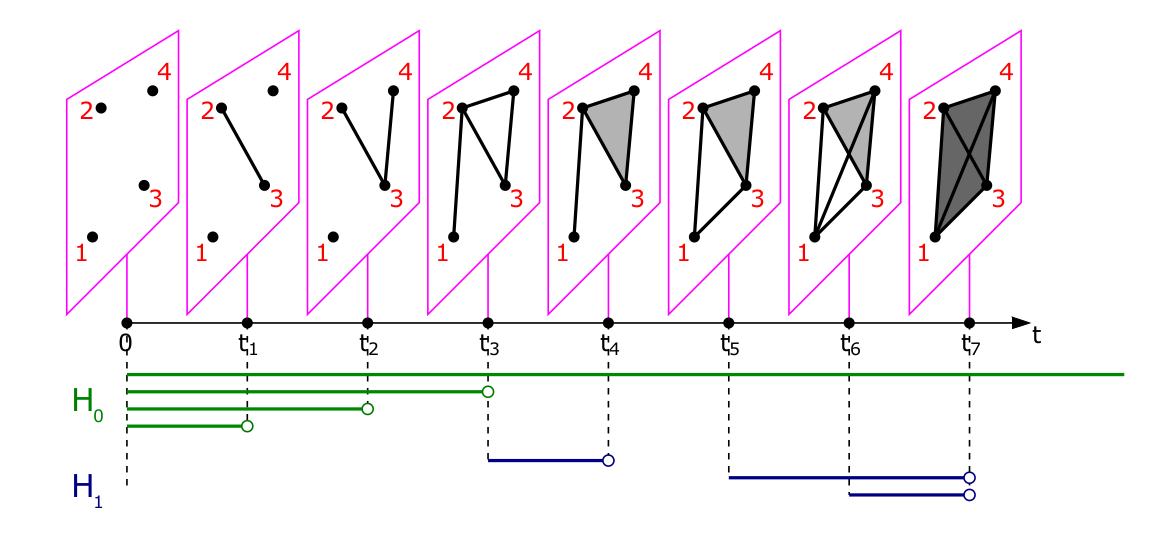
\includegraphics[width=\linewidth]{filtrationAyzenberg.png}
		\end{figure}
		\note{Радиусы шаров можно менять и получать (вообще говоря) разные комплексы. Это называют фильтрацией. Устойчивыми гомологиями называют набор гомологий для каждого комплекса в фильтрации. Внизу изображен баркод -- способ представления информации об устойчивых гомологиях. Баркод содержит отрезки, которые начинаются в тот момент времени, когда появился соответствующий цикл, и закачиваются тогда, когда соответствующий цикл исчез.}
		\end{frame}
		\begin{frame}
			\frametitle{Фильтрации и устойчивые гомологии}
			\begin{figure}
				\centering
				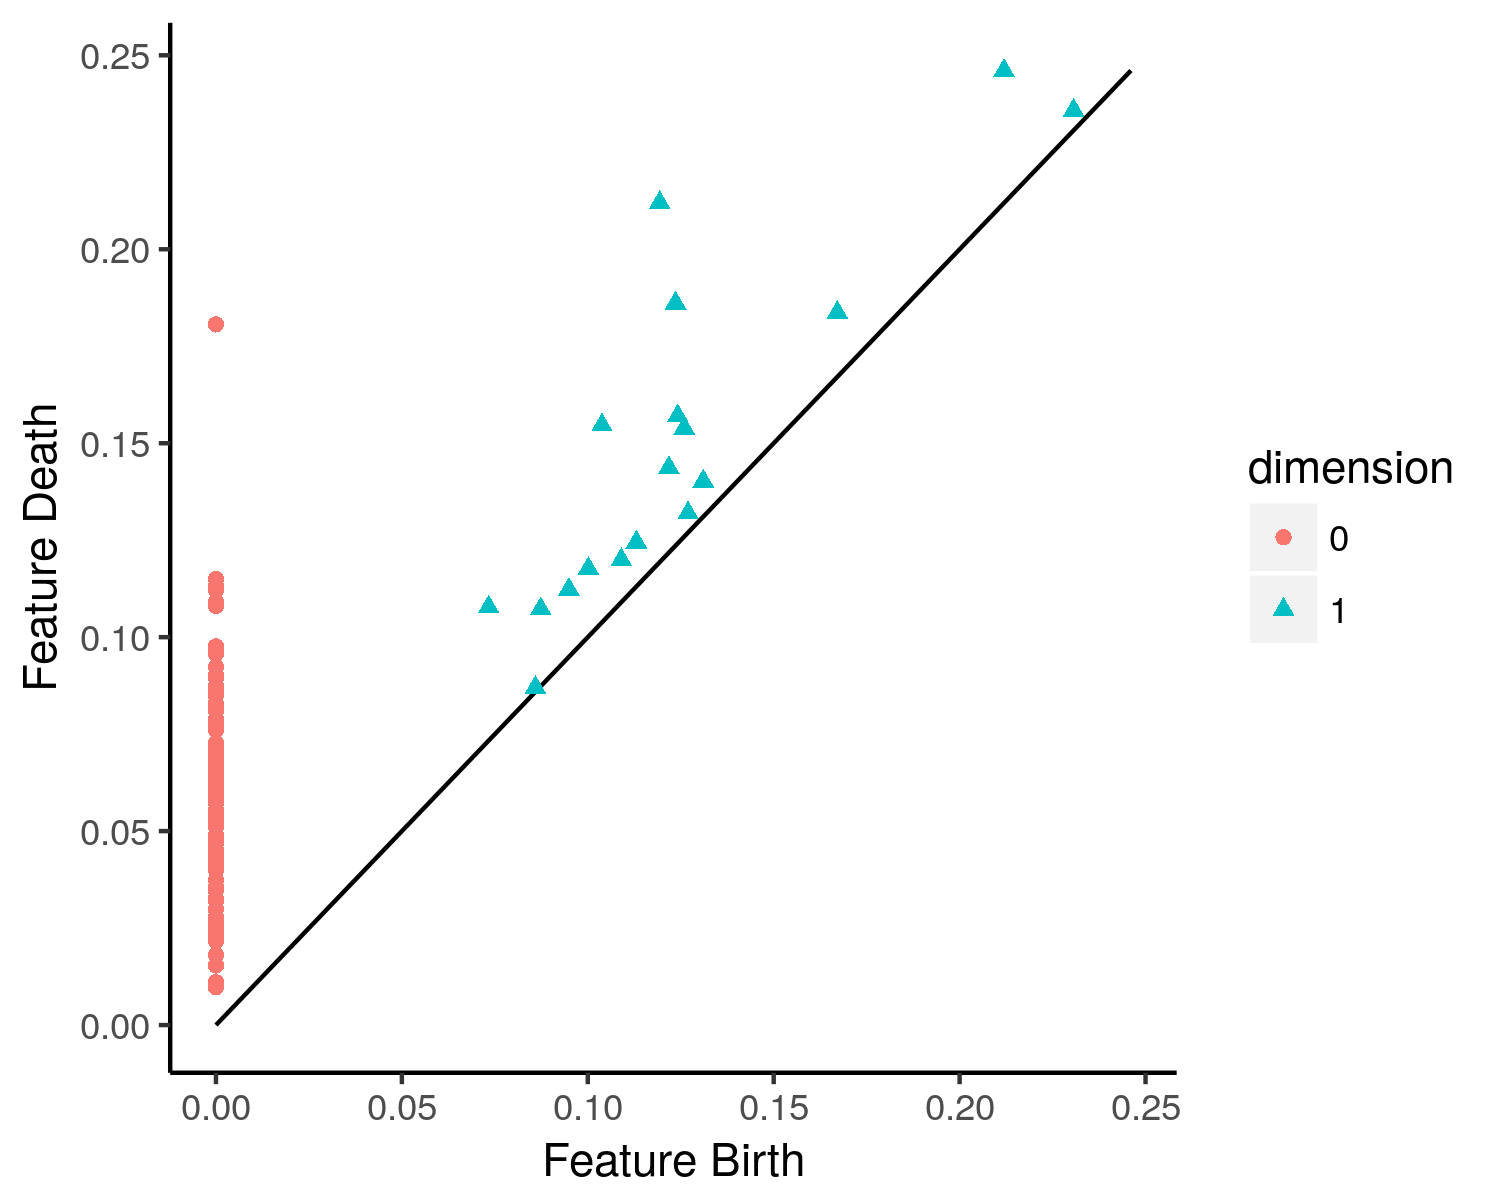
\includegraphics[width=0.6\linewidth]{persist_diag.png}
				\caption{Диаграмма персистентности}
			\end{figure}
				\note{Данную информацию можно представлять и другим способом -- в качестве т.н. диаграммы персистентности. Ось абсцисс -- время появления цикла, ось ординат -- время ее исчезновения. Таким образом каждая точка на диаграмме соответсвует некоторому циклу -- это как раз та информация, которую хотелось бы извлечь.}
		\end{frame}
		\subsection{Векторизация диаграмм персистентности}
		\begin{frame}
			\frametitle{Векторизация диаграмм персистентности}
			Диаграммы устойчивости с данной метрикой образуют метрическое пространство $\mathcal{D}$:
			\[
			W_p(B, B^{'}) = \inf\limits_{\gamma:B\to B^{'}} 
			\big( 
			\sum\limits_{u \in B} \norm{u - \gamma(u)}_\infty^p
			\big) ^{\frac{1}{p}}.
			\]
			
			%На множестве $\mathcal{D}$ диаграмм персистентности можно ввести структуру метрического пространства, однако для большинства алгоритмов машинного обучения и анализа данных требуется более сложная структура.
			
			%Можно векторизовать диаграмму, т.е. построить отображение $ \varphi: \mathcal{D} \to V $, где $V$ -- нормированное векторное пространство. Тогда диаграмме $B$ можно сопоставить число -- $\norm{\varphi(B)}$.
			{\it Векторизация диаграмм} -- это отображение $ \varphi: \mathcal{D} \to V $, где $V$ -- нормированное векторное пространство.
			\begin{figure}
				\centering
				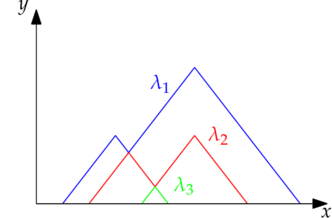
\includegraphics[width=0.5\linewidth]{persistent_landscape.png}
				\caption{График некоторой векторизации}
			\end{figure}
		\note{К сожалению, нельзя просто взять, и использовать методы машинного обучения на диаграмм устойчивости. Множество диаграмм образуют метрическое пространство, но многие модели требуют более сложную структуру. Поэтому, для того, чтобы использовать топологическую информацию, стараются сопоставить диаграмме некоторый вектор из нормированного пространства. Это называется векторизацией. Причем важно, чтобы векторизация была устойчива: чтобы небольшое изменение на диаграмме приводило к небольшому изменению вектора. Тогда, взяв норму вектора, можно сопоставить диаграмме некоторое число.}
		\end{frame}
	\section{Алгоритм классификации}
		\subsection{Алгоритм построения векторного представления}
		\begin{frame}
			%Построить фильтрацию для изображения можно различными методами. В настоящей работе было построено 20 разнообразных фильтрацией, для каждой из которых были получены $0$ и $1$ персистентные гомологии, из диаграмм которых было получено 14 признаков. Таким образом, для одной картинки было получено $20 \times 2 \times 14 = 560$ признаков.
			\frametitle{Алгоритм построения векторного представления}
			\begin{algorithm}[H]
				\normalsize
				\SetAlgoLined
				\KwData{Черное-белое изображение}
				\KwResult{Вектор размерности $d$}
				По изображению построить $n$ разных кубических фильтраций
				
				\ForEach{фильтрации}
				{найти ее $0$ и $1$ кубические гомологии
					
				 построить диаграмму устойчивости
			 		
			 	 посчитать $k$ разных векторных представлений
		 		
	 			} 
 				
 				Собрать $d = 2nk$ представлений в один вектор
				\note{В своей работе я реализовывал следующий алгоритм ... Построить фильтрацию для изображения можно различными методами. В настоящей работе было построено 20 разнообразных фильтрацией, для каждой из которых были получены $0$ и $1$ персистентные гомологии, из диаграмм которых было получено 14 признаков. Таким образом, для одной картинки было получено $20 \times 2 \times 14 = 560$ признаков.}
			\end{algorithm}
		\end{frame}
		\iffalse
		\begin{frame}
			\frametitle{Пайплайн используемого метода построения векторного представления}
			Построить фильтрацию для изображения можно различными методами. В настоящей работе было построено 20 разнообразных фильтрацией, для каждой из которых были получены $0$ и $1$ персистентные гомологии, из диаграмм которых было получено 14 признаков. Таким образом, для одной картинки было получено $20 \times 2 \times 14 = 560$ признаков.
			\begin{figure}
				\centering
				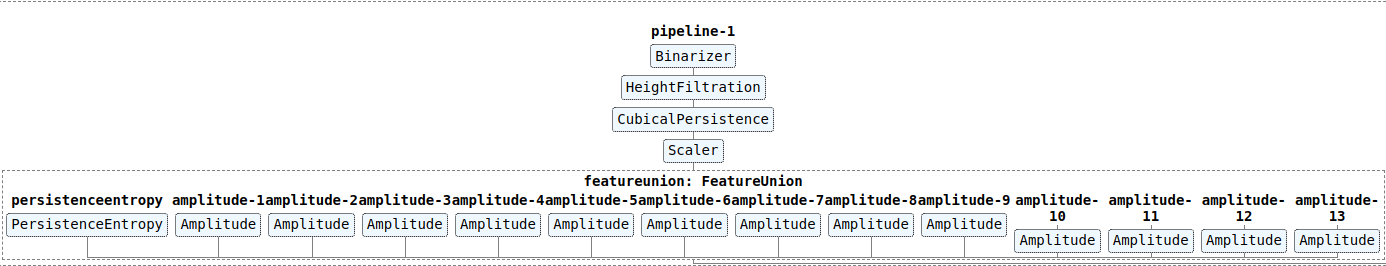
\includegraphics[width=\linewidth]{pipelineDiagram.png}
			\end{figure}
		\end{frame}
		\fi
		
		\begin{frame}
			\frametitle{Использованное ПО}
			\begin{columns}[T] % align columns
				\begin{column}{.25\textwidth}
					\color{red}\rule{\linewidth}{4pt}
					\normalsize
					\begin{itemize}
						\item Python
						\item Scikit-Learn
						\item Giotto-TDA
						\item NumPy
						\item Matplotlib
					\end{itemize}
				\end{column}%
				\hfill%
				\begin{column}{.74\textwidth}
					\begin{figure}
						\centering
						
\includegraphics[width=0.6\linewidth]{libraries.jpg}
					\end{figure}
				\end{column}%
			\end{columns}
		\note{Данный алгоритм был написан на Python. Для машинного обучения были использлваны ..., а для вычисления устойчивых гомологий ... . Из всегда датасета MNIST я использовал лишь малое число объектов -- 700 на трейне, 300 на тесте.}
		\end{frame}
		
		\begin{frame}
			\frametitle{Процесс получения векторного представления}
			\begin{figure}
				\centering
				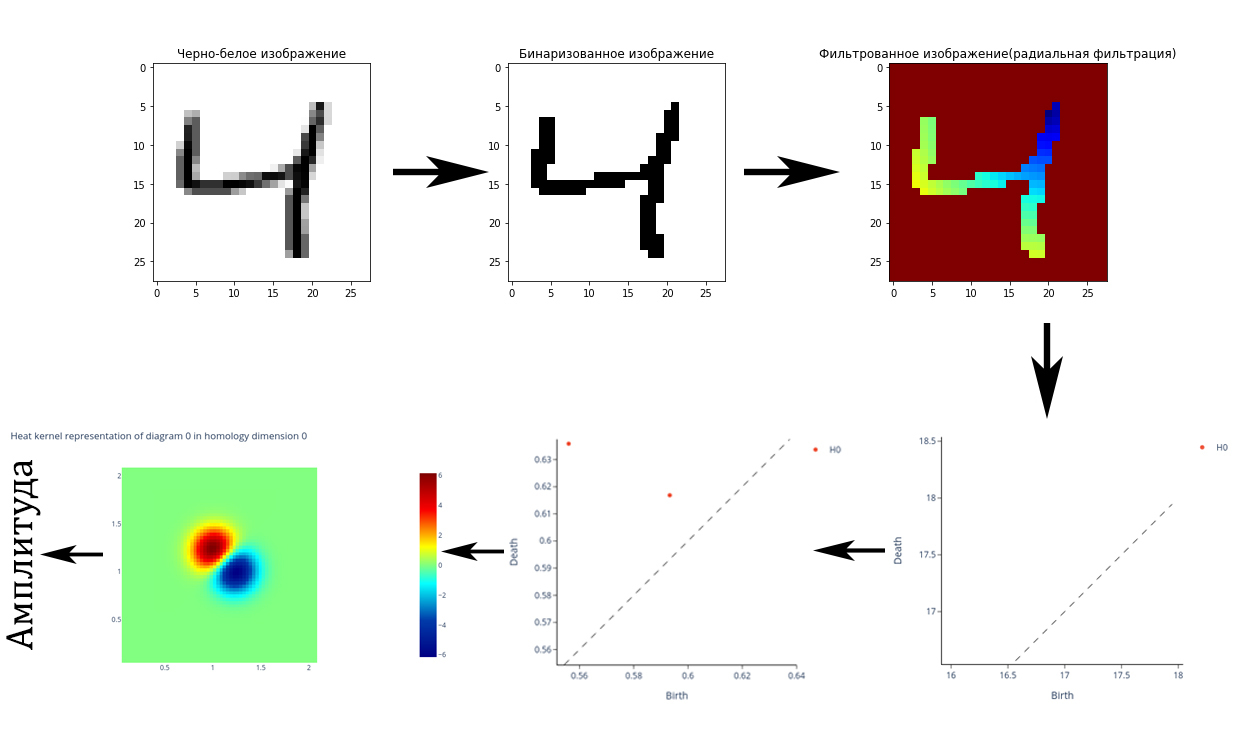
\includegraphics[width=\linewidth]{pipe.jpg}
			\end{figure}
		\note{На слайде изображено получение векторого представления для конкретного изображения...}
		\end{frame}
		\subsection{Полученные результаты}
		\begin{frame}
			\frametitle{Сравнение результатов различных методов машинного обучения}
			\begin{center}
				\begin{table}[!htbp]
					\centering
					\small
					\caption{Значения базовых моделей на тренировочной и тестовой выборках}	
					\label{tabl:baselines}
					\begin{tabularx}{\linewidth}{|X|X|X|}
					\hline
					Название модели & Значение на тренировочной выборке & Значение на тестовой выборке\\ \hline
					Логистическая регрессия & 0.989 & 0.903 \\
					\hline 
					Метод опорных векторов & 1.0 & 0.893 \\
					\hline
					Случайный лес & 1.0 & 0.89 \\
					\hline
					LightGBM & 1.0 & 0.9 \\
					\hline
					XGBoost & 1.0 & 0.883 \\
					\hline
					CatBoost & 1.0 & 0.893 \\ 
					\hline
					\end{tabularx}
				\end{table}
			\end{center}
		\note{Получив векторые представления для диаграмм, далее использовались методы машинного обучения для предсказания класса. Видно, что методы даже с неподобранными параметрами показывают очень хороший результат, при этом многие модели переобучаются.}
		\end{frame}
		\begin{frame}
			\frametitle{Сравнение результатов различных методов машинного обучения}
			\begin{center}
				\begin{table}[!htbp]
					\centering
					\small
					\caption{Значения наилучших моделей, полученных в результате подбора параметров поиском по сетке, на тренировочной и тестовой выборках}	
					\begin{tabularx}{\linewidth}{|X|X|X|}
						\hline
						Название модели & Значение на тренировочной выборке & Значение на тестовой выборке\\ \hline
						Логистическая регрессия & 0.911 & 0.917 \\
						\hline 
						Метод опорных векторов & 0.903 & 0.893 \\
						\hline
						Случайный лес & 0.88 & 0.87 \\
						\hline
						LightGBM & 0.908 & 0.917 \\
						\hline
						XGBoost & 0.907 & 0.897 \\ 
						\hline
						CatBoost & 1.0 & 0.927 \\ 
						\hline
					\end{tabularx}
					\label{tabl:gridsearch}
				\end{table}
			\end{center}
		\note{На данном слайде изображены модели с подобранными гиперпараметрами. Действительно, данные модели показывают очень неплохой результат точности, учитывая небольшую выборку. Вероятно многие признаки коррелируют друг с другом, поэтому с помощью случайного леса отранжируем признаки по важности и построим график точности моделей от числа признаков. Также сравним качество данных моделей с моделями, которые в качестве признаков рассматривают сами изображения, точнее их плоские представления. Такой вариант считается классическим}
		\end{frame}
		\begin{frame}
			\frametitle{Подбор гиперпараметров и отбор признаков}
			\begin{figure}
			\begin{subfigure}{0.48\textwidth}
				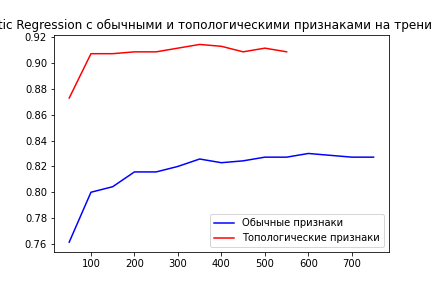
\includegraphics[width=\linewidth]{log_diff_features_train.png}
				\caption{Тренировочная выборка}
				\label{fig:1}
			\end{subfigure}%\hfil % <-- added
			\begin{subfigure}{0.48\textwidth}
				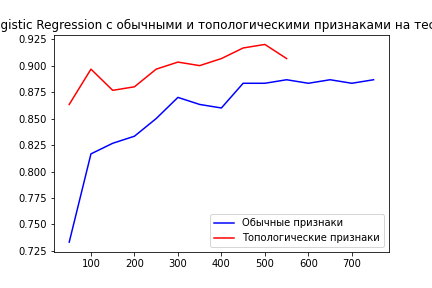
\includegraphics[width=\linewidth]{log_diff_features_test.png}
				\caption{Тестовая выборка}
				\label{fig:2}
			\end{subfigure}
			\caption{Логистическая регрессия}
			\end{figure}
		\note{Сравнивая с моделью с обычными признаками видно, что модель с топологическими признаками показывает более высокую точность. Помимо этого видно, что, скажем, первые 100 важных топ признаков, несут в себе больше информации, чем первые 100 обычных}
		\end{frame}
			\begin{frame}
				\frametitle{Подбор гиперпараметров и отбор признаков}
				\begin{figure}
					\begin{subfigure}{0.48\textwidth}
						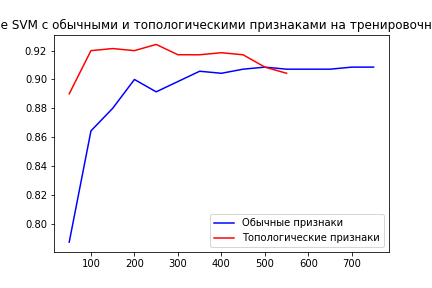
\includegraphics[width=\linewidth]{svm_diff_features_train.png}
						\caption{Тренировочная выборка}
						\label{fig:1}
					\end{subfigure}%\hfil % <-- added
					\begin{subfigure}{0.48\textwidth}
						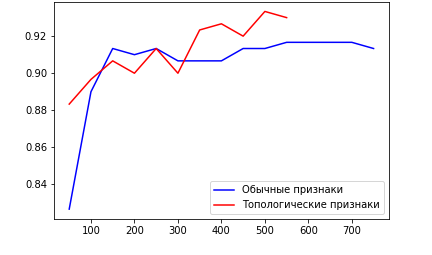
\includegraphics[width=\linewidth]{svm_diff_features_test.png}
						\caption{Тестовая выборка}
						\label{fig:2}
					\end{subfigure}
				\caption{Метод опорных векторов}
				\end{figure}
			\note{Похожая ситуация и с свм, хотя и менее наглядно. Видно, что в среднем имеется прирост точности у моделей с топологическими признаками, чем с обычными.}
			\end{frame}
			\begin{frame}
				\frametitle{Подбор гиперпараметров и отбор признаков}
				\begin{figure}
					\begin{subfigure}{0.48\textwidth}
						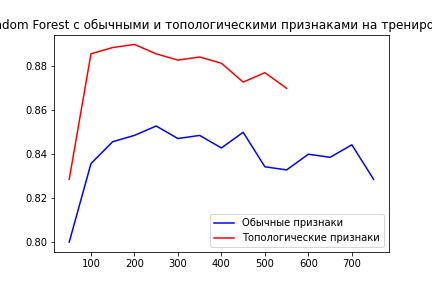
\includegraphics[width=\linewidth]{rf_diff_features_train.png}
						\caption{Тренировочная выборка}
						\label{fig:1}
					\end{subfigure}%\hfil % <-- added
					\begin{subfigure}{0.48\textwidth}
						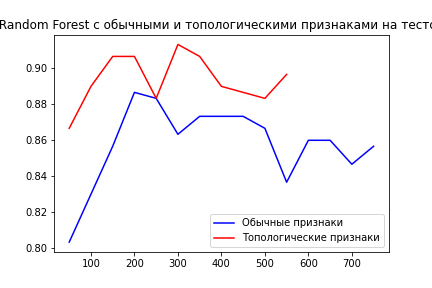
\includegraphics[width=\linewidth]{rf_diff_features_test.png}
						\caption{Тестовая выборка}
						\label{fig:2}
					\end{subfigure}
				\caption{Случайный лес}
				\end{figure}
			\note{Такая же картина и для случайного леса. Модели с топологическими признаками в целом требуется гораздо меньше признаков, чем обычно модели, и при этом она показывает стабильно более высокую точность. Таким образом, можно считать, что реализованный алгоритм является алгоритмом повышения размерности}
			\end{frame}
		
		\begin{frame}
			\frametitle{Первые несколько изображений, на которых ошибся классификатор}
			\begin{figure}[!htbp]
				\begin{center}
					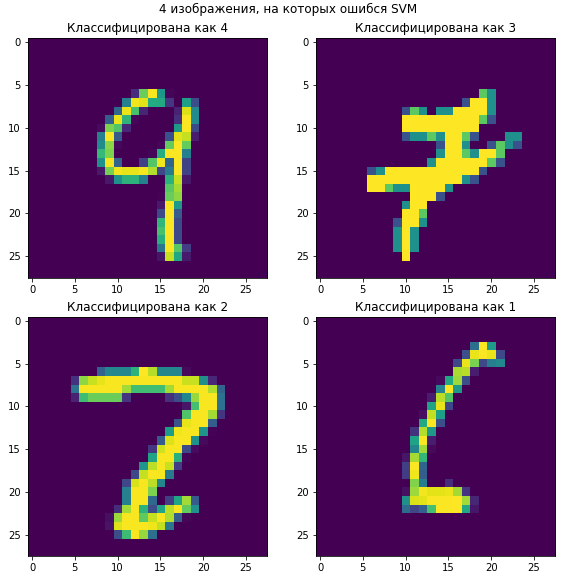
\includegraphics[width=0.5\textwidth]{missclassified.png}\\
					%\caption{Первые несколько изображений, на которых ошибся классификатор}
					\label{missclassified}
				\end{center}
			\end{figure}
		\note{Также интересно посмотреть, на каких изображениях ошибся классификатор. Видно, почему он некоторые изображения классифицировал именно так, как классифицировал, при этом видно, что эти изображения действительно очень сложно корректно классифицировать}
		\end{frame}
		
	\section{Заключение}
		\subsection{Результаты}
		\begin{frame}
			\frametitle{Результаты} % ОТДЕЛЬНО РЕЗУЛЬТАТЫ, ОТДЕЛЬНО ВЫВОДЫ
			\begin{itemize}
				\item В ходе данной работы был изучен теоретический материал по алгебраической и прикладной топологии и машинному обучению. 
				\item Было проведено сравнение пакетов топологического анализа данных.
				\item Был реализован алгоритм классификации датасета MNIST, который использовал только топологические характеристики рукописных цифр в качестве признаков.%, который выдавал высокий уровень точности.
				
				%\item В ходе данной работы было выявлено, что реализованный алгоритм является эффективным алгоритмом понижения размерности пространства признаков. 
				\item Было проведено сравнение моделей машинного обучения с разными признаками. %Было проведено сравнение с другими моделями машинного обучения, в результате которого было обнаружено, что реализованный алгоритм показывает более высокую точность классификации при меньшем числе признаков.
			\end{itemize}
		\note{Таким образом, в ходе данной бакалаврской работы было ...}
		\end{frame}
		
		\begin{frame}
			\frametitle{Выводы} % ОТДЕЛЬНО РЕЗУЛЬТАТЫ, ОТДЕЛЬНО ВЫВОДЫ
			\begin{itemize}
				\item Подход, основанный на топологических характеристиках данных, показал свою работоспособность на примере изображений.
				\item Реализованный алгоритм является эффективным алгоритмом понижения размерности пространства признаков: он показывает более высокую точность классификации при меньшем числе признаков. 
			\end{itemize}
		\note{В ходе данной работы были получены следующие выводы: }
		\end{frame}
	
		\begin{frame}%[allowframebreaks]
			\centering
			
			\begin{beamercolorbox}[sep=8pt,center,colsep=-4bp,rounded=true,shadow=true]{institute}
				\usebeamerfont{title}{Спасибо за внимание!}
			\end{beamercolorbox}
			
			\vskip1em\par
			
			\begin{beamercolorbox}[sep=8pt,left,colsep=-4bp,rounded=true,shadow=true]{date}
				\normalsize
				\usebeamerfont{date}{Мои публикации на данную тему:
				\nocite{*}
				\printbibliography	
			}
			\end{beamercolorbox}\vskip0.5em
		\note{Спасибо за внимание}
		\end{frame}
\end{document}